Im Youtube Video~\url{https://youtu.be/X_DdGRjtwAo} des Kanals
Stand-up Maths stellt Youtuber Matt Parker die folgende Frage
zu Würfelresultaten im Spiel Dungeons and Dragons.
Der Spieler wirft zwei Würfel mit $n$ Seiten
($n$ kann 4, 5, 6, 8, 10, 12 oder 20 sein).
Als Resultat zählt der grössere der beiden Würfel.
\begin{teilaufgaben}
\item
Wie gross ist die Wahrscheinchlichkeit für jedes der möglichen
Resultate $1,\dots,n$?
\item
Wie gross ist der Erwartungswert des Resultates?
\item
Geben Sie den numerischen Wert von $E(X)$ für $n=20$.
\ifthenelse{\boolean{pruefung}}{}{
\item
Verallgemeinern Sie das Problem auf $d=3$ Würfel.
}
\end{teilaufgaben}

\begin{hinweis}
Die folgenden Formeln können nützlich sein:
\begin{align*}
\sum_{k=1}^n k &= \frac{n(n+1)}{2}
&
\sum_{k=1}^n k^2 &= \frac{n(n+1)(2n+1)}{6}
&
\sum_{k=1}^n k^3 &= \frac{n^2(n+1)^2}{4}
\end{align*}
\ifthenelse{\boolean{pruefung}}{}{In der Prüfung war Teilaufgabe d)
nicht Bestandteil dieser Aufgabe.}
\end{hinweis}

\begin{loesung}
\begin{figure}
\centering

\definecolor{colorsix}{rgb}{1,0,0.2}
\definecolor{colorfive}{rgb}{1,0.6,0}
\definecolor{colorfour}{rgb}{0.8,1,0}
\definecolor{colorthree}{rgb}{0,0.6,0}
\definecolor{colortwo}{rgb}{0.2,0.6,1}
\definecolor{colorone}{rgb}{0,0,1}

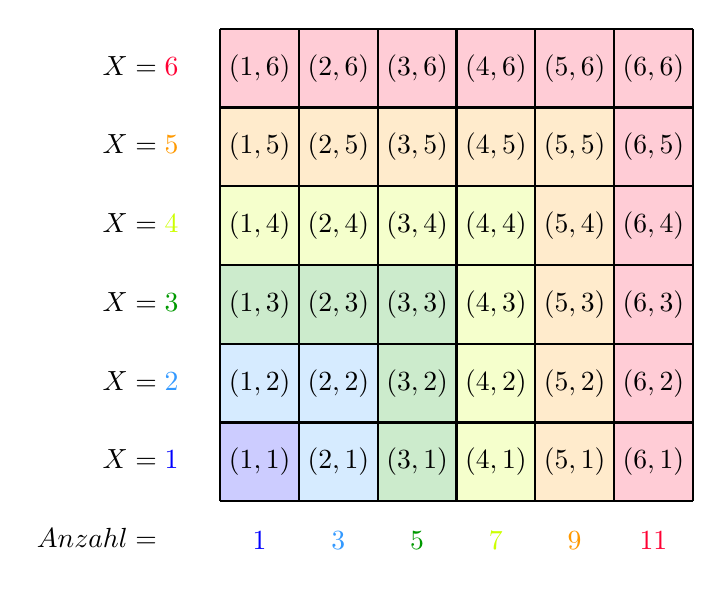
\begin{tikzpicture}[>=latex,thick]
\def\ds{1}
\def\wuerfelpaar#1#2{
	\node at ({(#1-0.5)*\ds},{(#2-0.5)*\ds}) {$(#1,#2)\mathstrut$};
}
\def\winkel#1#2{
	\fill[color=#2!20] (0,{(#1-1)*\ds})
		-- ({(#1-1)*\ds},{(#1-1)*\ds})
		-- ({(#1-1)*\ds},0)
		-- ({#1*\ds},0)
		-- ({#1*\ds},{#1*\ds})
		-- (0,{#1*\ds}) 
		-- cycle;
	\node at ({-0.4*\ds},{(#1-0.5)*\ds})
		[left] {$X={\color{#2}#1}\mathstrut$};
}
\def\anzahl#1#2{
	\node at ({((#1-0)*0.5)*\ds},{(-0.5*\ds)}) {${\color{#2}#1}$};
}
\winkel{6}{colorsix}            \anzahl{11}{colorsix}
\winkel{5}{colorfive}           \anzahl{9}{colorfive}
\winkel{4}{colorfour}           \anzahl{7}{colorfour}
\winkel{3}{colorthree}          \anzahl{5}{colorthree}
\winkel{2}{colortwo}            \anzahl{3}{colortwo}
\winkel{1}{colorone}            \anzahl{1}{colorone}
\node at ({-0.4*\ds},{(-0.5)*\ds})
	[left] {$\text{Anzahl}=\phantom{0}\mathstrut$};
\foreach \t in {0,...,6}{
	\draw ({\t*\ds},0) -- ({\t*\ds},{6*\ds});
	\draw (0,{\t*\ds}) -- ({6*\ds},{\t*\ds});
}
\foreach \x in {1,...,6}{
	\foreach \y in {1,...,6}{
		\wuerfelpaar{\x}{\y}
	}
}

\end{tikzpicture}
\caption{Mögliche Resultate beim Wurf zweier Sechserwürfel, wenn man nur
die grössere der beiden Augenzahlen zählt.
\label{40000051:fig}}
\end{figure}%
\begin{teilaufgaben}
\item
Seien $X_1$ und $X_2$ die Würfelresultate der einzelnen Würfel, dann
ist die Wahrscheinlichkeit der einzelnen Wert der Zufallsvariable
$X=\max(X_1,X_2)$ gesucht.
In Abbildung~\ref{40000051:fig} sind die möglichen Würfelresultate
dargestellt.
Es gibt $2k-1$ mögliche Arten, das Resultat $X=k$ zu erreichen.
Die Gesamtzahl der Würfelresultate ist $n^2$.
Die Wahrscheinlichkeit für das Resultat $X=k$ ist daher
\[
P(X=k) = \frac{2k-1}{n^2}.
\]
\item
Der Erwartungswert von $X$ ist
\begin{align}
E(X)
&=
\sum_{k=1}^n k\cdot P(X=k)
=
\sum_{k=1}^n \frac{k(2k-1)}{n^2}
=
\frac{1}{n^2} \biggl(2\sum_{k=1}^n k^2 - \sum_{k=1}^n k\biggr).
\notag
\intertext{Die Summen von $k$ und $k^2$ auf der rechten Seite können
in geschlossener Form ausgewertet werden, dies ergibt}
&=
\frac{1}{n^2}
\biggl(
2
\frac{n(n+1)(2n+1)}{6}
-
\frac{n(n+1)}2
\biggr)
=
\frac{1}{n^2}\biggl(
\frac{2n^3+3n^2+n}{3}
-
\frac{n^2+n}2
\biggr)
\notag
\\
&=
\frac{1}{n^2}\biggl(
\frac{4n^3+6n^2+2n}{6}
-
\frac{3n^2+3n}{6}
\biggr)
=
\frac{1}{n^2}\biggl(
\frac{4n^3+3n^2-n}{6}
\biggr)
\notag
\\
&=
\frac{2}{3}n
+
\frac{1}{2}
-
\frac{1}{6n}.
\label{40000051:resultatb}
\end{align}
\item
Für $n=20$ ist
$E(X) = \frac23\cdot 20 + \frac12 - \frac{1}{120}
=
13.825$.
\ifthenelse{\boolean{pruefung}}{
\qedhere
}{
\item
Zunächst muss wieder die Anzahl Möglichkeiten gefunden werden, wie
das Würfelresultat $X=k$ erreicht werden.
Es gibt $k^d$ Möglichkeiten für Würfelresultate, in denen kein
Würfel ein grösseres Resultat als $k$ anzeigt.
Daher gibt es genau $k^d-(k-1)^d$ Möglichkeiten, das Resultat $X=k$
zu erreichen und es folgt
\[
P(X) = \frac{k^d-(k-1)^d}{n^d}.
\]
Der Erwartungswert ist
\begin{align*}
E(X)
&=
\sum_{k=1}^n
k\cdot P(X=k)
=
\frac{1}{n^3}
\sum_{k=1}^n
k
\bigl(k^3-(k-1)^3\bigr)
=
\frac{1}{n^3}
\sum_{k=1}^n
\bigl(
3k^3-3k^2+k
\bigr)
\\
&=
\frac{1}{n^3}
\biggl(
3\frac{n^2(n+1)^2}{4}
-
3\frac{n(n+1)(2n+1)}{6}
+
\frac{n(n+1)}{2}
\biggr)
\\
&=
\frac{1}{n^3}
\biggl(
\frac{9}{12}(n^4+2n^3+n^2)
-
\frac{6}{12}(2n^3+3n^2+n)
+
\frac{6}{12}(n^2+n)
\biggr)
\\
&=
\frac{1}{12n^3}
\biggl(
9n^4 + 6n^3 - 3n^2 
\biggr)
\\
&=
\frac34n + \frac12 -\frac{1}{4n}.
\qedhere
\end{align*}
}
\end{teilaufgaben}
\end{loesung}

\begin{diskussion}
Man kann das Problem auch für eine beliebige Anzahl $d$ von Würfeln
lösen.
Die Wahrscheinlichkeit des Resultats $X=k$ ist bereits berechnet werden,
damit kann man den Erwartungswert als
\begin{align*}
E(X)
&=
\sum_{k=1}^n
k \cdot P(X=k)
=
\sum_{k=1}^n k\frac{k^d-(k-1)^d}{n^d}
=
\frac{1}{n^d}
\underbrace{\sum_{k=1}^n k(k^d-(k-1)^d)}_{\displaystyle = S_n}
\end{align*}
ansetzen.
Schreibt man die Summe als
\begin{align}
S_n
&=
n\cdot\bigl(n^d-(n-1)^d\bigr)
+
(n-1)\bigl((n-1)^d - (n-2)^d\bigr)
+
(n-2)\bigl((n-2)^d - (n-3)^d\bigr)
+
\dots
\notag
\\
&=
n^{d+1}
+
(-n+n-1)(n-1)^d
+
(-(n-1)+n-2)(n-2)^d
+
(-(n-2)+n-3)(n-3)^d
+\dots
\notag
\\
&=
n^{d+1}
-
(n-1)^d - (n-2)^d - \dots
\notag
\\
&=
n^{d+1}
-
\sum_{k=1}^{n-1} k^d
\label{40000051:summe}
\end{align}
aus, kann man erkennen, dass sich aufeinanderfolgende
Terme zum Teil wegheben.
Um $S_n$ zu berechnen, braucht man eine Formel für die Summe der
Potenzen $k^d$.
Dies leistet die Faulhabersche Formel, die man zum Beispiel
in der Wikipedia unter
\url{https://de.wikipedia.org/wiki/Faulhabersche_Formel}
finden kann.
Wir verwenden sie in der Form
\begin{equation}
\sum_{k=1}^{n-1} k^d
=
\frac{1}{d+1}
\sum_{j=0}^d\binom{d+1}{j}B_j n^{d+1-j}.
\label{40000051:faulhaber}
\end{equation}
Darin sind $B_j$ die Bernoullischen Zahlen, $B_0=1$, $B_1=-\frac12$, $B_2=\frac16$ \dots

Setze man 
\eqref{40000051:faulhaber}
in
\eqref{40000051:summe}
ein, findet man
\begin{align*}
S_n
&=
n^{d+1}
-\frac1{d+1}\biggl(
\binom{d+1}{0} B_0n^{d+1}
+
\binom{d+1}{1} B_1n^{d+1-1}
+
\sum_{j=2}^d \binom{d+1}{j} B_j n^{d+1-j}
\biggr)
\\
&=
n^{d+1}-\frac{n^{d+1}}{d+1}
+
\frac{1}{2}n^d
-
\frac{1}{d+1}\sum_{j=2}^d\binom{d+1}{j}B_jn^{d+1-j}
\\
&=
n^{d+1}\frac{d}{d+1}
+
\frac{1}{2}n^d
-
\frac{1}{d+1}\sum_{j=2}^d\binom{d+1}{j}B_jn^{d+1-j}.
\end{align*}
Nach Division durch $n^{d+1}$ findet man den Erwartungswert
\[
E(X)
=
\frac{S_n}{n^d}
=
\frac{d}{d+1}
n
+
\frac12
-
\frac{1}{d+1}\sum_{j=2}^d\binom{d+1}{j}B_jn^{1-j}.
\]
Zur Kontrolle untersuchen wir den Fall $d=2$.
In diesem Fall hat die Summe auf der rechten Seite nur einen einzigen
Term, in dem $B_2=\frac16$ vorkommt.
Sein Wert ist
\[
\frac{1}{d+1}\sum_{j=2}^d\binom{d+1}{j}B_jn^{1-j}
=
\frac{1}{3}\binom{3}{2}B_2n^{-1}
=
\frac{1}{3}\cdot 3\cdot \frac1{6n}
=
\frac{1}{6n},
\]
was mit dem dritten Term in
\eqref{40000051:resultatb}
übereinstimmt.
\end{diskussion}


